\chapter{Results\label{results}}
% information about chapter
This chapter employes the data extracted from the set of primary literature, available in this thesis' repository \citep{mscthesis} under the name of \texttt{stage1-licenses.md}, utilizing the methods outlined in \hyperref[methods]{Chapter 2} to address the research questions. Firstly, a summary of the general statistics collected and aggregated from the studies is presented. Following that, an analysis of the data is performed to provide answers to each of the research questions.

% note about publication year and literature amount
To begin with, the publication year was not limited and could not have been limited in a rigorous way. Almost all of the public software licenses came from different sources although they were listed in the five license listing sites. To give a rough estimate, one of the earliest public software license aiming for legal compliance was the original GPL from 1989 \citep{license-history}. The search was carried out by web scraping all of the licenses from the five license listing sites without any filters to the attributes of the licenses. The initial search results included 1057 public licenses, but after the exclusion and quality criteria of software-only license scope, the final resulting dataset was reached.

% statistical overview
Given the large starting dataset, a simple statistical overview of the literature was generated and is presented in \hyperref[fig:3-1]{Figure 3.1} and \hyperref[fig:3-2]{Figure 3.2} with the full list of literature available in this thesis' repository \citep{mscthesis} under the name of \texttt{stage1-licenses.md}.
\begin{figure}
	\centering
	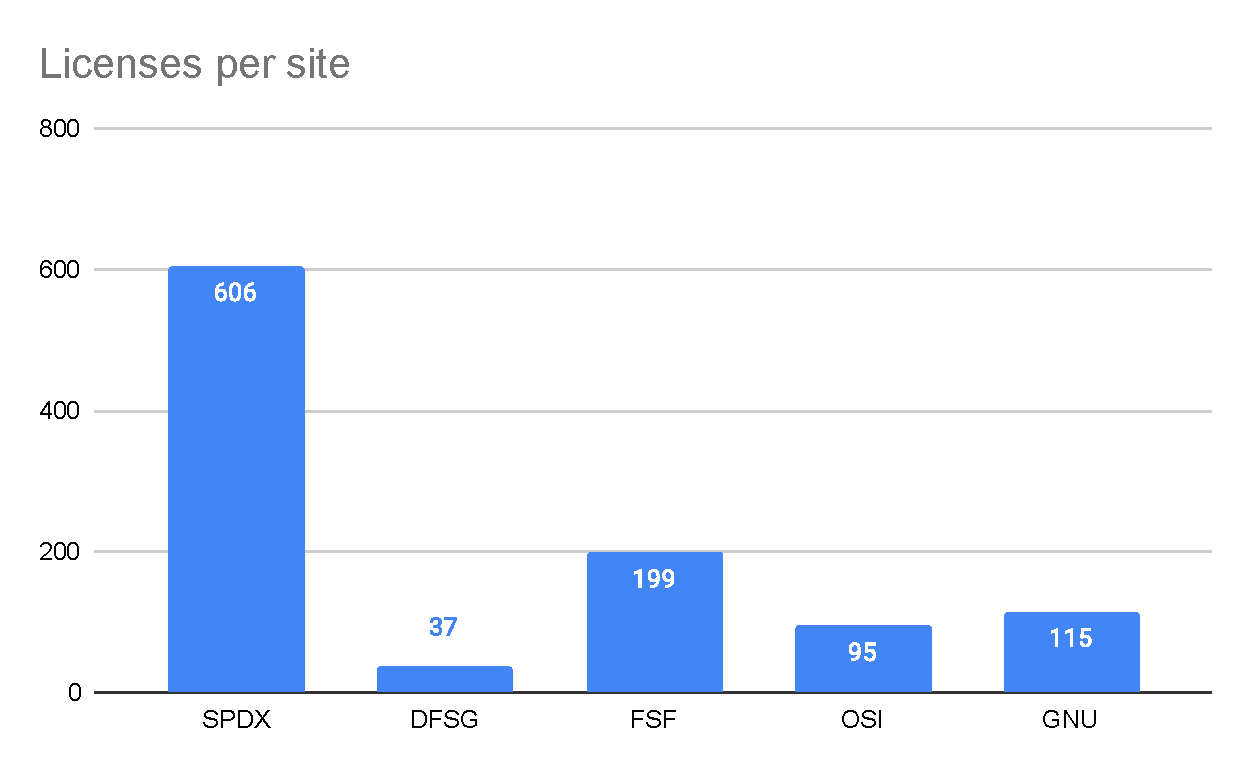
\includegraphics[scale=0.76]{figures/figure-3-1.pdf}
	\caption{Statistics about the original 1057 licenses}
	\label{fig:3-1}
\end{figure}
\begin{figure}
	\centering
	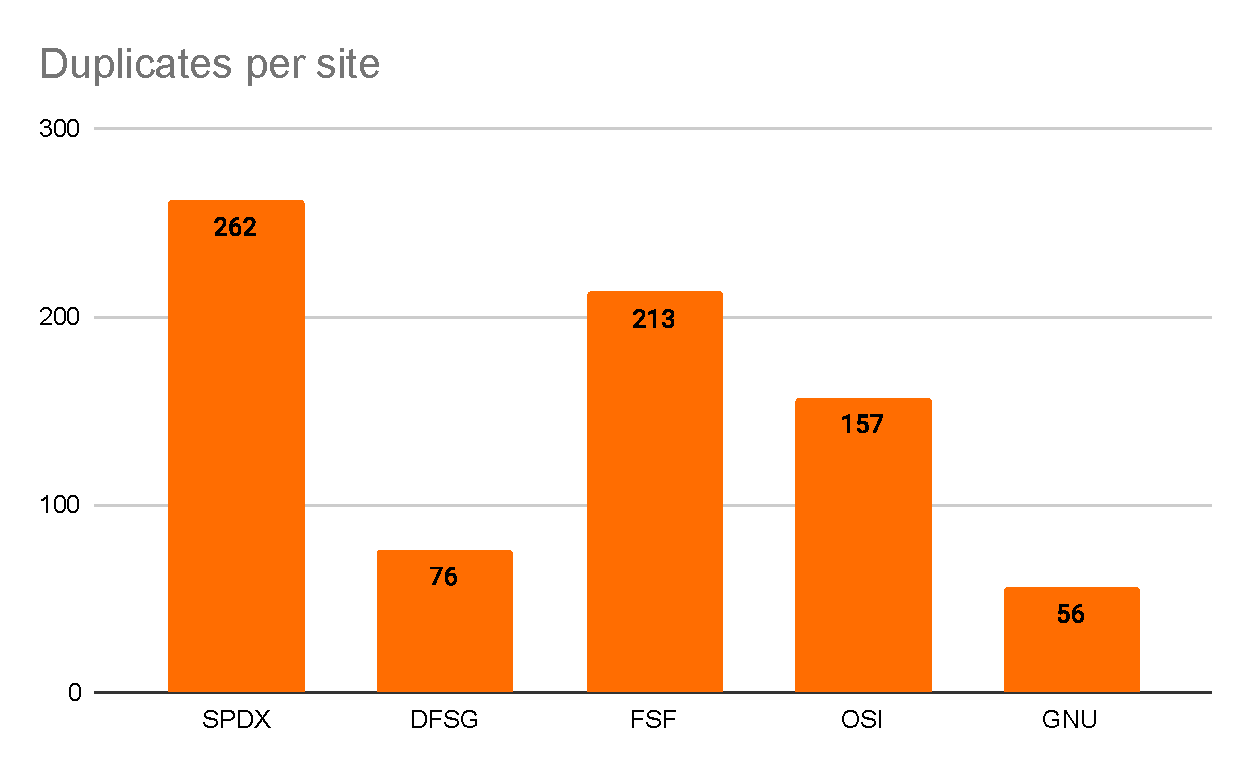
\includegraphics[scale=0.76]{figures/figure-3-2.pdf}
	\caption{Duplicate statistics about the original 1057 licenses}
	\label{fig:3-2}
\end{figure}
The statistics highlight some immediate observations, such as the volume differences between the five sites and how the initial volume doesn't correlate to the amount of duplicate one site holds compared to the four others.

% recap search process
After establishing the quasi-gold standard and completing the preliminary study review outlined in \hyperref[methods]{Chapter 2}, we systematically searched for relevant literature using the five license listing sites. The resulting search findings were filtered through a set of inclusion/exclusion criteria, followed by an extensive evaluation of quality before the final step of manual review. The final collection of literature consisted of 594 licenses, for which we obtained and reviewed the complete texts while completing the data extraction form as presented in \hyperref[table:extraction]{Table 2.1}. To enhance transparency of the process, \hyperref[fig:3-3]{Figure 3.3} illustrates the progression of literature through each stage.
\begin{figure}
	\centering
	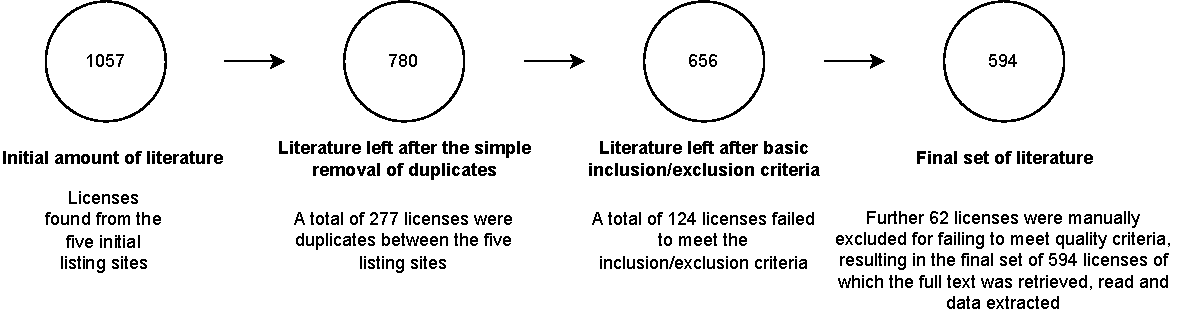
\includegraphics[scale=0.8]{figures/figure-3-3.pdf}
	\caption{Number of literature per step of data collection}
	\label{fig:3-3}
\end{figure}
We observed the number of literature acquired is adequate to gain an representative overview of the field, which we will explore further in this chapter.

After this overview let us take a look into the specific research questions and their answers.

\section{Five license listing sites and their licenses (RQ1)}

% notable observation on a few different types of licenses
Only license listing site that didnt give headache was spdx
% the other type of licenses
% research literature shows in between type
% some other note and findign about the five listing sites licenses
\section{Duplicates in license listing sites (RQ2)}
% note the amount of duplicates per site
% note some other thing about this particular finding
\section{Total amount of public software licenses (RQ3)}
% note the amount of software licenses in appendix c

% notable observation on legal validity
A notable observation regarding the total amount of existing public software licenses is that many of the licenses might not be considered legally valid in any court and many of them do not even try to be legally valid in the court. An example of the former, possibly not court-fireproof software license is the \texttt{MIT}. The breach of the license is not meant to be settled in court but rather just agreeing developer to developer that the distributed software contains MIT -licensed source code. Some examples of the latter include \texttt{Beerware} and \texttt{JSON} from which the former recommends buying a licensor a cold beverage and the latter forbids the use of software to evil purposes. 


\textcolor{red}{it's good to note that when bumping into the missing license of attpubliclicense which was from gnu, it turned out that the license listing site doesnt state the license content whatsoever. i had to just put the comment of the license into manual licenses.}

\textcolor{red}{mention how many missing/manual licenses there were. and from which site respectively}

\textcolor{red}{it could be a good idea to mention how many missing licenses came out of which sites. or it could be out of scope. i can just make a validity threat and say with face value that most of them were from FSF, GNU in that order. Python license seems just straight up an accident on FSF's side. scope is not to fix the documentation problems of the 5 organizations though so I'll leave it just like that and mention the possibility of it being just an accident.}

\textcolor{orange}{the eye-pass of 87 excluded licenses included cal1.0 and cal-combined which seem to need to be included. made inclusions.txt to manually include them although containing the words creative commons, since those license texts were licensed themselves with creative commons. will eyeball the stage-2 shortcodes as well just to see anything i know by heart is not public software license. cc-by-sa-japanese was included so i had to make a manual exclusions.txt to manually mark licenses that are not public software licenses.}

\textcolor{orange}{we relaized that we were trying to fix the problem we were trying to give awareness to in the thesis by trying to distinguish automatically what is a public software license in the sea of 600+ licenses.}